% !TeX program = xelatex
% 高一数学 · 4.2.2 指数函数的图象和性质
% 编译：xelatex 指数函数的图象和性质.tex（连续两遍）
\documentclass[aspectratio=169,11pt,t,fleqn]{ctexbeamer}

\usepackage{amsmath,amssymb}
\usepackage{tabularx}% 自动调整表格宽度
\usepackage{booktabs}% 制作专业的三线表
\usepackage{graphicx}% 插入与处理图形
\usepackage{multirow}% 合并多行单元格
\usepackage{colortbl}
\usepackage{caption}
\captionsetup[figure]{name=图}
\setbeamertemplate{caption}[numbered]% 图形自动编号

\usepackage{pgfplots}
\pgfplotsset{compat=1.18}

% ---- 思源字体 ----
\setCJKmainfont{Source Han Serif SC}[BoldFont={Source Han Serif SC Bold}]
\setCJKsansfont{Source Han Sans SC}[BoldFont={Source Han Sans SC Bold}]
\usefonttheme[stillsansseriflarge]{serif}
% ---- 配色（教材蓝）----
\definecolor{mainblue}{RGB}{23,103,171}
\definecolor{lightblue}{RGB}{222,235,247}
\definecolor{accent}{RGB}{196,60,50}
\definecolor{dotpink}{RGB}{214,60,120}

\definecolor{xyyg}{cmyk}{0,1,1,0.45}
\definecolor{xyyg_gold}{cmyk}{0,0.35,0.75,0.05}
\definecolor{xyyg_blue}{cmyk}{0.6,0.35,0.0,0.4}
\definecolor{xyyg_darkblue}{cmyk}{1.0,0.6,0.0,0.5}
\definecolor{xyyg_gray}{cmyk}{0.0,0.0,0.08,0.55}
\definecolor{xyyg_dirt}{cmyk}{0.0,0.2,0.35,0.3}

\setbeamertemplate{theorems}[numbered]% 定理自动编号
\newtheorem{instance}{例}% 新建例题环境
\setcounter{instance}{2}% 本节教材为例 3、例 4
\BeforeBeginEnvironment{instance}{%
	\setbeamercolor{block title}{bg=xyyg_darkblue,fg=white}
	\setbeamercolor{block body}{bg=xyyg_blue!10}
}
\AfterEndEnvironment{instance}{
	\setbeamercolor{block title}{bg=xyyg,fg=white}
	\setbeamercolor{block body}{bg=xyyg!10}
}

% ---- 指数函数图象通用样式 ----
\pgfplotsset{
  expaxis/.style={
    width=6.4cm, height=5.2cm,
    axis lines=center,
    xmin=-3.2, xmax=3.2, ymin=-0.4, ymax=8.6,
    xtick={-3,-2,-1,0,1,2,3},
    ytick={1,2,3,4,5,6,7,8},
    xlabel={$x$}, ylabel={$y$},
    label style={font=\small},
    xlabel style={above},
    tick label style={font=\footnotesize},
    samples=200,
    domain=-3:3,
  },
}

\usetheme{Boadilla}
\usecolortheme{whale}

\setbeamercolor{structure}{fg=xyyg}
\setbeamercolor{alerted text}{fg=accent}

\setbeamercolor{palette primary}{use=structure,fg=white,bg=structure.fg}
\setbeamercolor{palette secondary}{use=structure,fg=white,bg=structure.fg!70!cyan}
\setbeamercolor{palette tertiary}{use=structure,fg=white,bg=structure.fg!20!black}
\setbeamercolor{palette quaternary}{fg=white,bg=structure.fg!85!black}

\AtBeginDocument{
  \setbeamercolor{block title alerted}{fg=white, bg=structure.fg!80}
  \setbeamercolor{block body alerted}{fg=black, bg=structure!10}
  \setbeamercolor{block title example}{fg=white, bg=green!50!black}
  \setbeamercolor{block body example}{fg=black, bg=green!10}
  \setbeamercolor{block title}{bg=xyyg,fg=white}
  \setbeamercolor{block body}{bg=xyyg!10}
  \setbeamertemplate{enumerate items}[default]
  \setbeamertemplate{itemize items}[ball]
}

\usepackage[most]{tcolorbox}
\tcbuselibrary{,}
\newtcolorbox{summarybox}[1][]{
	colback=purple!10,enhanced, drop fuzzy shadow=gray,
	colframe=purple!70!black,
	fonttitle=\bfseries,
	title=#1,
	arc=1mm,
	boxrule=0pt,
	left=2mm, right=2mm, top=2mm, bottom=2mm,
}

% ---- 表格表头底色 ----
\setbeamercolor{tablehead}{bg=xyyg!80,fg=black}

\title[指数函数的图象和性质]{4.2 指数函数}
\subtitle{4.2.2 指数函数的图象和性质}
\author[好好学习，努力向上]{}
\date{2026-11-24}

\begin{document}

% ============ 标题页 ============
\begin{frame}
  \titlepage
\end{frame}

% ============ 研究思路 ============
\begin{frame}{研究思路}
  类比研究幂函数性质的过程和方法，进一步研究指数函数：\alert{先画出指数函数的图象，然后借助图象研究指数函数的性质}。

  \vspace{0.8em}
  先从最简单的函数 $y=2^x$ 开始。
\end{frame}

% ============ 表 4.2-2：y=2^x 对应值表 ============
\section{画图象}
\begin{frame}{表 4.2-2\quad 函数 $y=2^x$ 的对应值表}
  \centering
  \renewcommand{\arraystretch}{1.2}
  \begin{tabular}{|c|c|}
    \hline
    \rowcolor{xyyg!60}
    \textbf{$x$} & \textbf{$y=2^x$} \\
    \hline
    $-2$    & $0.25$ \\
    \hline
    $-1.5$  & $0.35$ \\
    \hline
    $-1$    & $0.50$ \\
    \hline
    $-0.5$  & $0.71$ \\
    \hline
    $0$     & $1$ \\
    \hline
    $0.5$   & $1.41$ \\
    \hline
    $1$     & $2$ \\
    \hline
    $1.5$   & $2.83$ \\
    \hline
    $2$     & $4$ \\
    \hline
  \end{tabular}

  \vspace{0.6em}
  \small 完成上表后，用\alert{描点法}即可画出函数 $y=2^x$ 的图象。
\end{frame}

% ============ 图 4.2-4：y=2^x ============
\begin{frame}{图 4.2-4\quad 函数 $y=2^x$ 的图象}
  \begin{columns}
    \column{0.48\textwidth}
    \centering
    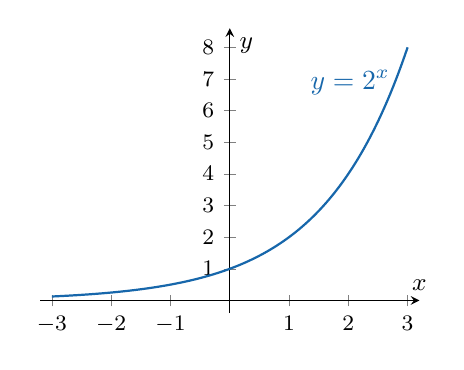
\begin{tikzpicture}[baseline=(current bounding box.north)]
      \begin{axis}[expaxis]
        \addplot[mainblue, thick, domain=-3:3] {2^x};
        \node[mainblue, anchor=south west] at (axis cs:1.2,6.2) {$y=2^x$};
      \end{axis}
    \end{tikzpicture}\\[2pt]
    图 4.2-4

    \column{0.52\textwidth}
    \begin{itemize}
      \item 图象经过点 $(0,1)$；
      \item 图象位于 $x$ 轴上方，函数值恒为正；
      \item 从左到右\alert{上升}，函数单调递增。
    \end{itemize}
  \end{columns}
\end{frame}

% ============ 探究：y=(1/2)^x ============
\begin{frame}{探究\quad $y=\left(\dfrac12\right)^x$ 的图象}
  \begin{block}{探究}
    画出函数 $y=\left(\dfrac12\right)^x$ 的图象，并与函数 $y=2^x$ 的图象进行比较，它们有什么关系？能否利用函数 $y=2^x$ 的图象，画出函数 $y=\left(\dfrac12\right)^x$ 的图象？
  \end{block}

  \vspace{0.6em}
  因为
  \[
    y=\left(\frac12\right)^x=2^{-x},
  \]
  点 $(x,y)$ 与点 $(-x,y)$ 关于 $y$ 轴对称，所以函数 $y=2^x$ 图象上任意一点 $P(x,y)$ 关于 $y$ 轴的对称点 $P_1(-x,y)$ 都在函数 $y=\left(\dfrac12\right)^x$ 的图象上，反之亦然。
\end{frame}

% ============ 图 4.2-5：两函数对称 ============
\begin{frame}{图 4.2-5\quad 关于 $y$ 轴对称}
  \begin{columns}
    \column{0.55\textwidth}
    \centering
    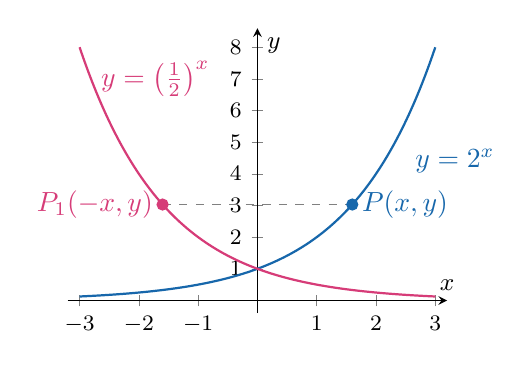
\begin{tikzpicture}[baseline=(current bounding box.north)]
      \begin{axis}[expaxis,clip=false]
        \addplot[mainblue, thick] {2^x};
        \addplot[dotpink, thick] {0.5^x};
        \node[mainblue, anchor=west] at (axis cs:2.5,4.4) {$y=2^x$};
        \node[dotpink, anchor= west] at (axis cs:-2.8,7) {$y=\left(\frac12\right)^x$};
        % 对称点 P 与 P1
        \addplot[only marks, mark=*, mainblue, mark size=2pt] coordinates {(1.6,3.03)};
        \addplot[only marks, mark=*, dotpink, mark size=2pt] coordinates {(-1.6,3.03)};
        \node[mainblue, anchor=west] at (axis cs:1.6,3.03) {$P(x,y)$};
        \node[dotpink, anchor=east] at (axis cs:-1.6,3.03) {$P_1(-x,y)$};
        \addplot[gray, dashed] coordinates {(-1.6,3.03) (1.6,3.03)};
      \end{axis}
    \end{tikzpicture}\\[2pt]
    图 4.2-5

    \column{0.45\textwidth}
    \begin{block}{结论}
      底数互为倒数的两个指数函数，图象关于\alert{$y$ 轴对称}。
    \end{block}
    根据这种对称性，就可以利用一个函数的图象，画出另一个函数的图象。
  \end{columns}
\end{frame}

% ============ 探究：多个底数 ============
\begin{frame}{探究\quad 选取若干底数画图观察}
  \begin{block}{探究}
    选取底数 $a$（$a>0$，且 $a\neq1$）的若干个不同的值，在同一直角坐标系内画出相应指数函数的图象。观察这些图象的位置、公共点和变化趋势，它们有哪些共性？由此你能概括出指数函数 $y=a^x$（$a>0$，且 $a\neq1$）的值域和性质吗？
  \end{block}

  \vspace{0.6em}
  如图 4.2-6，选取底数 $a$ 的若干值画图后可以发现：指数函数 $y=a^x$ 的图象按底数 $a$ 的取值，可分为 \alert{$0<a<1$} 和 \alert{$a>1$} 两种类型，因此它的性质也分这两种情况进行研究。
\end{frame}

% ============ 图 4.2-6：多底数图象 ============
\begin{frame}{图 4.2-6\quad 若干指数函数的图象}
  \centering
  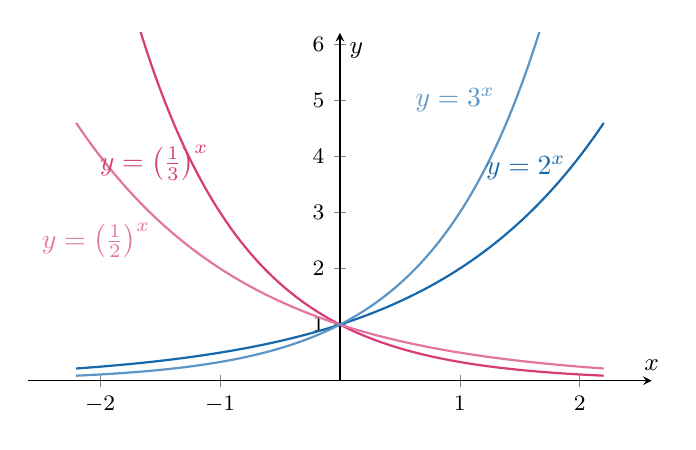
\begin{tikzpicture}
    \begin{axis}[
      width=9.5cm, height=6.0cm,
      axis lines=center,
      xmin=-2.6, xmax=2.6, ymin=0, ymax=6.2,
      xtick={-2,-1,0,1,2}, ytick={1,2,3,4,5,6},
      xlabel={$x$}, ylabel={$y$},
      label style={font=\small},
      xlabel style={above},
      tick label style={font=\footnotesize},
      samples=200, domain=-2.2:2.2,
    ]
      % 0<a<1：底数越小，图象越陡（递减）
      \addplot[dotpink, thick] {1/3^x};
      \addplot[dotpink!70, thick] {0.5^x};
      % a>1：底数越大，图象越陡（递增）
      \addplot[mainblue, thick] {2^x};
      \addplot[mainblue!70, thick] {3^x};
      \node[dotpink, anchor=south] at (axis cs:-1.55,3.4) {$y=\left(\frac13\right)^x$};
      \node[dotpink!70, anchor=east] at (axis cs:-1.5,2.5) {$y=\left(\frac12\right)^x$};
      \node[mainblue!70, anchor=west] at (axis cs:0.55,5) {$y=3^x$};
      \node[mainblue, anchor=south] at (axis cs:1.55,3.4) {$y=2^x$};
    \end{axis}
  \end{tikzpicture}\\[2pt]
  图 4.2-6
\end{frame}

% ============ 表 4.2-3：图象和性质 ============
\section{归纳性质}
\begin{frame}{表 4.2-3\quad 指数函数的图象和性质}
  \centering
  \small
  \renewcommand{\arraystretch}{1.8}
  \begin{tabular}{|c|c|c|}
    \hline
    \rowcolor{xyyg!60}
    & \textbf{$0<a<1$} & \textbf{$a>1$} \\
    \hline
    \textbf{图象}
    &
      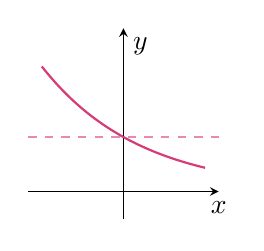
\begin{tikzpicture}[baseline=(current bounding box.center)]
        \begin{axis}[width=4cm, height=4cm, axis lines=center, clip=false,
          xmin=-1.4,xmax=1.4,ymin=-0.5,ymax=3.0,xlabel=$x$,ylabel=$y$,
          xlabel style={below},
          xtick=\empty,ytick=\empty, samples=100, domain=-1.2:1.2]
          \addplot[dotpink, thick] {0.5^x};
          \draw[dotpink!60, dashed] (-1.4,1) -- (1.4,1);
        \end{axis}
      \end{tikzpicture}
    &
      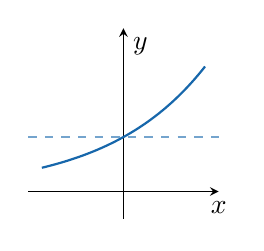
\begin{tikzpicture}[baseline=(current bounding box.center)]
        \begin{axis}[width=4cm, height=4cm, axis lines=center, clip=false,
          xmin=-1.4,xmax=1.4,ymin=-0.5,ymax=3.0,xlabel=$x$,ylabel=$y$,
          xlabel style={below},
          xtick=\empty,ytick=\empty, samples=100, domain=-1.2:1.2]
          \addplot[mainblue, thick] {2^x};
          \draw[mainblue!60, dashed] (-1.4,1) -- (1.4,1);
        \end{axis}
      \end{tikzpicture} \\
    \hline
    \textbf{定义域} & \multicolumn{2}{c|}{$\mathbb{R}$} \\
    \hline
    \textbf{值域} & \multicolumn{2}{c|}{$(0,+\infty)$} \\
    \hline
    \multirow{2}{*}{\textbf{性质}}
      & 过定点 $(0,1)$，即 $x=0$ 时 $y=1$
      & 过定点 $(0,1)$，即 $x=0$ 时 $y=1$ \\
    \cline{2-3}
      & （2）\alert{减函数}
      & （2）\alert{增函数} \\
    \hline
  \end{tabular}
\end{frame}

% ============ 性质补充 ============
\begin{frame}{性质补充\quad 图象与 $y=1$ 的位置关系}
  \begin{columns}
    \column{0.5\textwidth}
    \centering
    \textbf{$0<a<1$（减函数）}\\[4pt]
    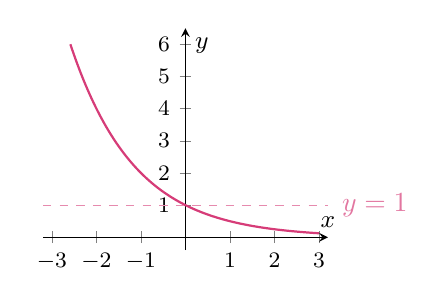
\begin{tikzpicture}
      \begin{axis}[expaxis, ymax=6.5, width=5.2cm, height=4.4cm, clip=false]
        \addplot[dotpink, thick,domain=-{ln(6)/ln(2)}:3] {0.5^x};
        \draw[dotpink!60, dashed] (-3.2,1) -- (3.2,1);
        \node[dotpink!70, anchor=west] at (axis cs:3.3,1) {$y=1$};
      \end{axis}
    \end{tikzpicture}
    \begin{itemize}\small
      \item $x<0$ 时，$y>1$；
      \item $x=0$ 时，$y=1$；
      \item $x>0$ 时，$0<y<1$。
    \end{itemize}

    \column{0.5\textwidth}
    \centering
    \textbf{$a>1$（增函数）}\\[4pt]
    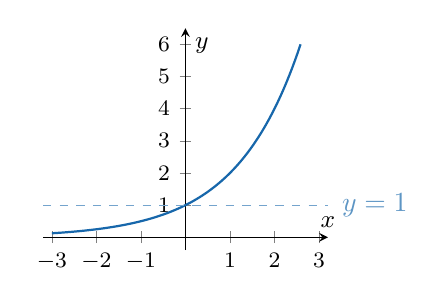
\begin{tikzpicture}
      \begin{axis}[expaxis, ymax=6.5, width=5.2cm, height=4.4cm, clip=false]
        \addplot[mainblue, thick,domain=-3:{ln(6)/ln(2)}] {2^x};
        \draw[mainblue!60, dashed] (-3.2,1) -- (3.2,1);
        \node[mainblue!70, anchor=west] at (axis cs:3.3,1) {$y=1$};
      \end{axis}
    \end{tikzpicture}
    \begin{itemize}\small
      \item $x<0$ 时，$0<y<1$；
      \item $x=0$ 时，$y=1$；
      \item $x>0$ 时，$y>1$。
    \end{itemize}
  \end{columns}
\end{frame}

% ============ 例 3 ============
\section{例题分析}
\begin{frame}{}
  \begin{instance}
    比较下列各题中两个值的大小：
    \begin{enumerate}[(\arabic*)]
      \item $1.7^{2.5}$，$1.7^{3}$；
      \item $0.8^{-\sqrt{2}}$，$0.8^{-\sqrt{3}}$；
      \item $1.7^{0.3}$，$0.9^{3.1}$。
    \end{enumerate}
  \end{instance}

  \vspace{0.3em}
  \small\textbf{分析：}对于 (1)(2)，要比较的两个值可以看作一个指数函数的两个函数值，可直接利用指数函数的单调性进行比较；对于 (3)，$1.7^{0.3}$ 和 $0.9^{3.1}$ 不能看作某一个指数函数的两个函数值，可以利用函数 $y=1.7^x$ 和 $y=0.9^x$ 的单调性，以及“$x=0$ 时 $y=1$”这一性质把它们联系起来。
\end{frame}

% ============ 例 3 解答 ============
\begin{frame}{例 3\quad 解答}
  \small
  \textbf{解：}

  \textbf{(1)} $1.7^{2.5}$ 和 $1.7^{3}$ 可看作函数 $y=1.7^x$ 当 $x$ 分别取 $2.5$ 和 $3$ 时所对应的两个函数值。

  因为底数 $1.7>1$，所以指数函数 $y=1.7^x$ 是\alert{增函数}。

  因为 $2.5<3$，所以 $\;1.7^{2.5}<1.7^{3}$。

  \vspace{0.6em}
  \textbf{(2)} 同 (1) 理，因为 $0<0.8<1$，所以指数函数 $y=0.8^x$ 是\alert{减函数}。

  因为 $-\sqrt{2}>-\sqrt{3}$，所以 $\;0.8^{-\sqrt{2}}<0.8^{-\sqrt{3}}$。

  \vspace{0.6em}
  \textbf{(3)} 由指数函数的性质知
  \[
    1.7^{0.3}>1.7^{0}=1,\qquad
    0.9^{3.1}<0.9^{0}=1,
  \]
  所以 $\;1.7^{0.3}>0.9^{3.1}$。
\end{frame}

% ============ 例 3 方法小结 ============
\begin{frame}{例 3\quad 方法小结}
  \begin{alertblock}{方法要点}
    利用指数函数的单调性，通过自变量的大小关系可以判断相应函数值的大小关系：
  \end{alertblock}

  \begin{enumerate}[(1)]
    \item \textbf{同底数}：直接构造指数函数，比较指数大小，依据单调性判断；
    \item \textbf{不同底数、不同指数}：找中间量（通常取 $1$，即 $a^0$）分别比较，再传递大小关系。
  \end{enumerate}
\end{frame}

% ============ 例 4 ============
\begin{frame}{}
  \begin{instance}
    如图 4.2-7，某城市人口呈指数增长。
    \begin{enumerate}[(\arabic*)]
      \item 根据图象，估计该城市人口每翻一番所需的时间（倍增期）；
      \item 该城市人口从 $80$ 万人开始，经过 $20$ 年会增长到多少万人？
    \end{enumerate}
  \end{instance}

  \vspace{0.3em}
  \small\textbf{分析：}
  (1) 因为该城市人口呈指数增长，而同一指数函数的倍增期是相同的，所以可以从图象中选取适当的点计算倍增期。

  (2) 要计算 $20$ 年后的人口数，关键是要找到 $20$ 年与倍增期的数量关系。
\end{frame}

% ============ 图 4.2-7：人口增长 ============
\begin{frame}{图 4.2-7\quad 某城市人口指数增长}
  \begin{columns}
    \column{0.58\textwidth}
    \centering
    \begin{tikzpicture}[baseline=(current bounding box.north)]
      \begin{axis}[
        width=7.0cm, height=5.2cm,
        axis lines=center,
        xmin=0, xmax=85, ymin=0, ymax=88,
        xtick={0,10,20,30,40,50,60,70,80},
        ytick={10,20,30,40,50,60,70,80},
        xlabel={$x$/年}, ylabel={$y$/万人},
        label style={font=\small},
        xlabel style={above},
        tick label style={font=\footnotesize},
        grid=both, grid style={gray!20},
        samples=200, domain=0:80,
      ]
        % 倍增期 20 年：y=5·2^(x/20)，x=20 时 10 万，x=40 时 20 万
        \addplot[dotpink, thick] {5*2^(x/20)};
      \end{axis}
    \end{tikzpicture}\\[2pt]
    图 4.2-7

    \column{0.42\textwidth}
    \small
    图象过点 $(20,10)$、$(40,20)$，人口由 $10$ 万人增长到 $20$ 万人所用时间约为 $20$ 年。
  \end{columns}
\end{frame}

% ============ 例 4 解答 ============
\begin{frame}{例 4\quad 解答}
  \small
  \textbf{解：}

  \textbf{(1)} 观察图 4.2-7，发现该城市人口经过 $20$ 年约为 $10$ 万人，经过 $40$ 年约为 $20$ 万人，即由 $10$ 万人口增加到 $20$ 万人口所用的时间约为 $20$ 年，所以该城市人口每翻一番所需的时间约为 \alert{$20$ 年}。

  \vspace{0.8em}
  \textbf{(2)} 因为倍增期为 $20$ 年，所以每经过 $20$ 年，人口将翻一番。因此，从 $80$ 万人开始，经过 $20$ 年，该城市人口大约会增长到
  \[
    80\times 2=160\ \text{万人}.
  \]
\end{frame}

% ============ 练习 ============
\section{课堂练习}
\begin{frame}{练习}
  \begin{enumerate}
    \item 在同一直角坐标系中画出函数 $y=3^x$ 和 $y=\left(\dfrac13\right)^x$ 的图象，并说明它们的关系。
    \item 比较下列各题中两个值的大小：
      \[
        \text{(1) }6^{\sqrt2},\ 7^{\sqrt2};\qquad
        \text{(2) }0.3^{-3.5},\ 0.3^{-2.3};\qquad
        \text{(3) }1.2^{0.5},\ 0.5^{1.2}.
      \]
    \item 体内癌细胞初期增加得很缓慢，但到了晚期就急剧增加，画一幅能反映体内癌细胞数量随时间变化的示意图。
  \end{enumerate}
\end{frame}

% ============ 练习 1 解答 ============
\begin{frame}{练习 1\quad 解答}
  \begin{columns}
    \column{0.55\textwidth}
    \centering
    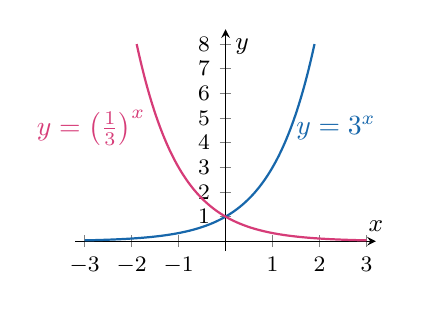
\begin{tikzpicture}[baseline=(current bounding box.north)]
      \begin{axis}[expaxis, width=5.4cm, height=4.4cm,clip=false,]
        \addplot[mainblue, thick,domain=-3:{log2(8)/log2(3)}] {3^x};
        \addplot[dotpink, thick,domain=-{log2(8)/log2(3)}:3] {1/3^x};
        \node[mainblue, anchor=west,] at (axis cs:1.3,4.6) {$y=3^x$};
        \node[dotpink, anchor=east] at (axis cs:-1.5,4.6) {$y=\left(\frac13\right)^x$};
      \end{axis}
    \end{tikzpicture}\\[2pt]
    $y=3^x$ 与 $y=\left(\frac13\right)^x$

    \column{0.45\textwidth}
    \small
    因为
    \[
      \left(\frac13\right)^x=3^{-x},
    \]
    所以点 $(x,y)$ 与点 $(-x,y)$ 关于 $y$ 轴对称。

  \vspace{0.3em}
    两个函数的图象\alert{关于 $y$ 轴对称}：$y=3^x$ 是增函数，$y=\left(\dfrac13\right)^x$ 是减函数，它们都过定点 $(0,1)$。
  \end{columns}
\end{frame}

% ============ 练习 2 解答 ============
\begin{frame}{练习 2\quad 解答}
  \small
  \textbf{解：}

  \textbf{(1)} $6^{\sqrt2}$ 与 $7^{\sqrt2}$ 指数相同，比较底数。在指数函数中，当指数 $\sqrt2>0$ 时，底数越大，幂越大；也可借助幂函数 $y=x^{\sqrt2}$（在 $x>0$ 时递增）判断。

  因为 $6<7$，$\sqrt2>0$，所以 $\;6^{\sqrt2}\alert{<}7^{\sqrt2}$。

  \vspace{0.6em}
  \textbf{(2)} $0.3^{-3.5}$ 和 $0.3^{-2.3}$ 可看作函数 $y=0.3^x$ 的两个函数值。因为 $0<0.3<1$，所以 $y=0.3^x$ 是\alert{减函数}。

  因为 $-3.5<-2.3$，所以 $\;0.3^{-3.5}\alert{>}0.3^{-2.3}$。

  \vspace{0.6em}
  \textbf{(3)} 找中间量 $1$：
  \[
    1.2^{0.5}>1.2^{0}=1,\qquad
    0.5^{1.2}<0.5^{0}=1,
  \]
  所以 $\;1.2^{0.5}\alert{>}0.5^{1.2}$。
\end{frame}

% ============ 练习 3 解答 ============
\begin{frame}{练习 3\quad 解答：癌细胞数量随时间变化示意图}
  \begin{columns}
    \column{0.55\textwidth}
    \centering
    \begin{tikzpicture}[baseline=(current bounding box.center)]
      \begin{axis}[
        width=6.6cm, height=5.0cm,
        axis lines=center,
        xmin=-2, xmax=10, ymin=-2, ymax=9,
        xtick=\empty, ytick=\empty,
        xlabel={时间}, ylabel={癌细胞数量},
        label style={font=\small},
        xlabel style={below },
        samples=200, domain=0:9,
      ]
        % 初期缓慢、晚期急剧增加：指数增长曲线
        \addplot[dotpink, thick] {0.6*1.28^x};
      \end{axis}
    \end{tikzpicture}

    \column{0.45\textwidth}
    \small
    初期数量增长平缓，随时间推移增长速度越来越快，曲线呈\alert{指数上升（下凸）}形态，与 $a>1$ 的指数函数 $y=a^x$ 的图象特征一致。
  \end{columns}
\end{frame}

% ============ 小结 ============
\begin{frame}{小结}
  \begin{block}{本节要点}
    \begin{enumerate}[(1)]
      \item \textbf{图象}：指数函数 $y=a^x$（$a>0$，且 $a\neq1$）的图象恒在 $x$ 轴上方，过定点 $(0,1)$；底数互为倒数的两个图象关于 $y$ 轴对称。
      \item \textbf{定义域与值域}：定义域为 $\mathbb{R}$，值域为 $(0,+\infty)$。
      \item \textbf{单调性}：$a>1$ 时为增函数；$0<a<1$ 时为减函数。
      \item \textbf{应用}：利用单调性比较幂的大小；利用指数增长模型分析倍增期等实际问题。
    \end{enumerate}
  \end{block}
\end{frame}

% ============ 布置作业 ============
\begin{frame}{布置作业}
  \begin{summarybox}[作业：]
    \begin{enumerate}[(1)]
      \item P118 练习 1、2、3；
      \item P118---119 习题 4.2\quad 5---10。
    \end{enumerate}
  \end{summarybox}
\end{frame}

\end{document}
